\documentclass[a4paper,12pt]{article}

% --- Essentiële Packages voor jouw project ---
\usepackage[dutch]{babel}          % Voor Nederlandstalige titels en afbreking
\usepackage[utf8]{inputenc}        % Voor speciale tekens
\usepackage[T1]{fontenc}
\usepackage{amsmath, amssymb}      % Voor al je wiskundige formules (warmtebalans)
\usepackage{geometry}              % Om je marges in te stellen
\geometry{margin=2.5cm}
\usepackage{graphicx}              % Voor het invoegen van je plannen en technische fiches
\usepackage{booktabs}              % Voor professionele tabellen (zoals je debieten)
\usepackage{tabularx} 
\usepackage[table]{xcolor}% Voor tabellen die automatisch schalen naar paginabreedte
\usepackage{siunitx}               % Super handig voor eenheden zoals m³/h of °C
\usepackage{placeins}              % De figuren binnnen de hoofdstukken blijven (Floatbarrier)
\sisetup{
  output-decimal-marker = {,},
  per-mode = fraction % <--- Dit zorgt voor de horizontale breukstreep
}
% Type,Commando,Resultaat
   % Alleen eenheid,\unit{\cubic\meter\per\hour},m³/h
    %Getal + eenheid,\qty{225}{\cubic\meter\per\hour},225 m³/h
    %Temperatuur,\qty{20}{\celsius},20 °C
    %Alleen getal,"\num{1234,56}","1.234,56"

\usepackage{float}
\usepackage{fancyhdr}              % Voor de UGent-stijl headers en footers
\usepackage{hyperref}              % Voor een klikbare inhoudsopgave
\usepackage{caption}               % Voor mooie bijschriften bij je figuren
\usepackage[parfill]{parskip}  % Zorgt voor witruimte tussen alinea's ipv inspringen
\usepackage{pdfpages}
\usepackage{adjustbox}

% --- Start van het document ---
\begin{document}

% Titelpagina (vrij in te vullen naar je voorbeeld)
\begin{titlepage}
    \centering
    {\scshape\LARGE Universiteit Gent \par}
    \vspace{1cm}
    {\scshape\Large Projectoefening Technische Installaties 2026\par}
    \vspace{1.5cm}
    {\huge\bfseries Installatieconcept Ham \par}
    \vspace{2cm}
    {\Large Groep 40\par}
    \vfill
    {\large \today \par}
\end{titlepage}

\tableofcontents % Je automatische inhoudstafel!
\newpage

\section{Inleiding}
\subsection{Toelichting Ontwerp}
Deze rijwoning maakt deel uit van een masterplan waarbij deze als units naast elkaar geplaatst werden, voor deze opdracht werd voor een unit gekozen die langs beide zijden buren heeft. De woning van 500m² is ontworpen als een cohousing waarbij er 2 gezinnen van 4 een gemeenschappelijke living delen, maar voor de rest gescheiden kunnen wonen. In het midden van het ontwerp bevindt zich een vide die van bovenuit daglicht tot in living brengt. Het gebouw wordt begrensd door klassieke spouwmuren met een beige gevelsteen.
\subsection{Plannen}
\begin{figure}[H]
    \centering
    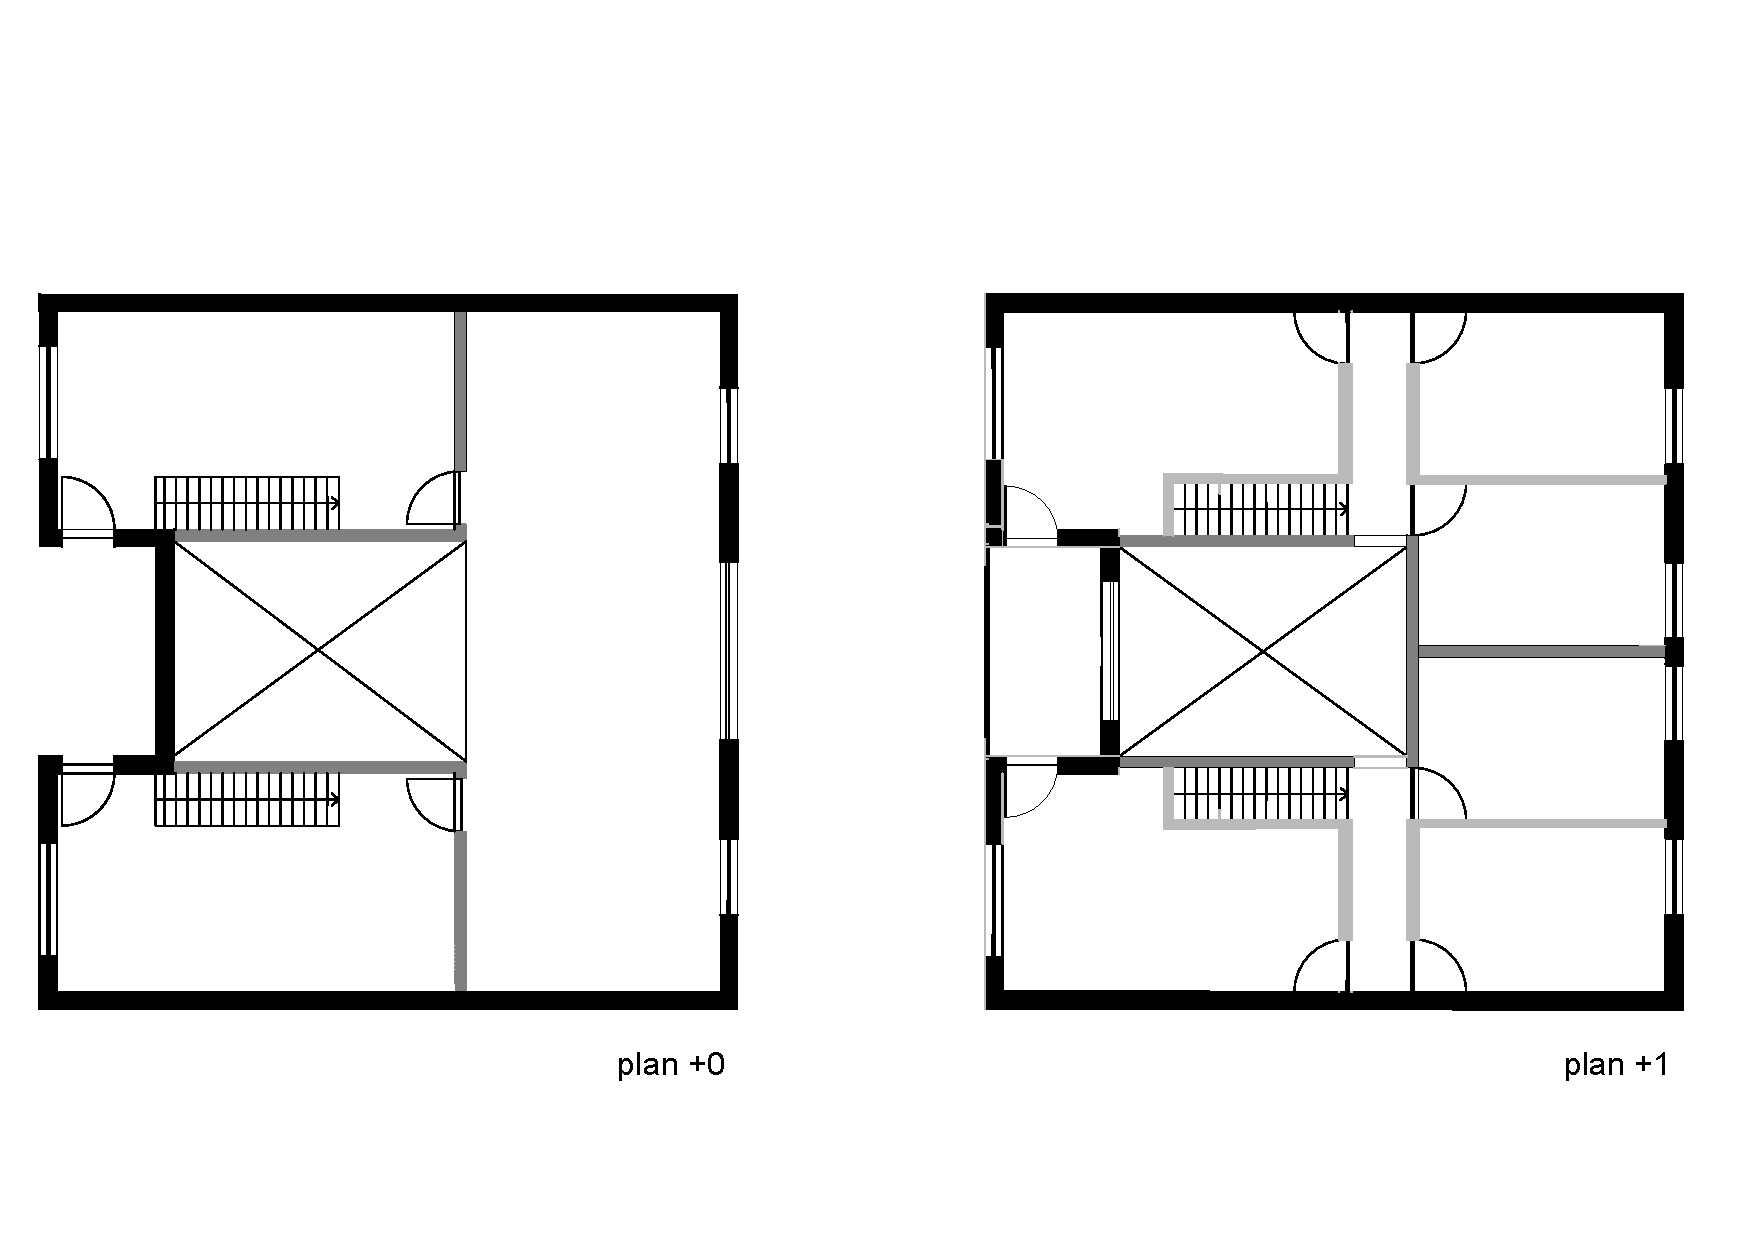
\includegraphics[width=1\linewidth]{figuren/TIG-plannen-woning-Layout3.pdf}
    \caption{plannen woning}
    \label{fig:plannen}
\end{figure}

\section{Plaatsing Technische Ruimte}
In ons huidig ontwerp stond nog geen technische ruimte hierbij hebben we gekozen om de technische ruimte te plaatsen in de vide. Hierdoor staat de ruimte mooi gecentreerd in de woning wat handig is voor de plaatsing van de meeste installaties. Daarnaast zitten we ook nog eens dicht bij de badkamers waardoor het sanitair warm water hier snel kan geraken. 
\subsection{Inplanting}
\begin{figure}[H]
    \centering
    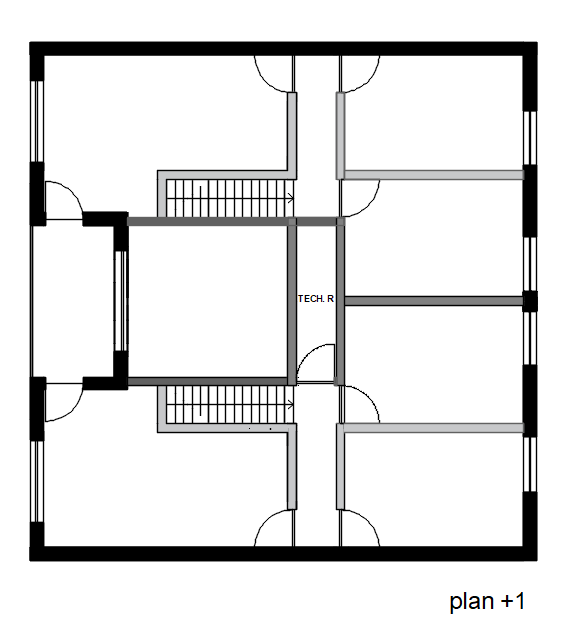
\includegraphics[width=0.5\linewidth]{figuren/TECHR.png}
    \caption{Implanting}
    \label{fig:plannen2}
\end{figure}

\section{Ventilatieconcept}

\subsection{Keuze ventilatiesysteem}
Voor dit project is de keuze gevallen op een mechanisch balansventilatiesysteem met warmteterugwinning (systeem D). Dit systeem garandeert een gecontroleerde toe- en afvoer van lucht, wat resulteert in een optimale en betrouwbare binnenluchtkwaliteit. De keuze wordt sterk gemotiveerd door de hoge energie-efficiëntie van de warmtewisselaar en het vermijden van ongewenste koudeval bij de toevoerpunten, wat het thermisch comfort aanzienlijk verhoogt. (dit zouk nog wat veranderen)

\subsection{Ontwerpdebieten}
De ontwerpdebieten voor de ventilatie zijn bepaald op basis van de geldende EPB-normering voor residentiële gebouwen. De algemene rekenregel stelt dat het nominale debiet ($q_{v, \text{nom}}$) berekend wordt in functie van de vloeroppervlakte ($A$) van de desbetreffende ruimte, namelijk \qty{3,6}{\cubic\meter\per\hour} per vierkante meter. Dit theoretische debiet wordt vervolgens afgetoetst aan de wettelijk vastgelegde minimum- en maximumwaarden per ruimtetype.

De gehanteerde formule voor het basisdebiet is:
\begin{equation}
    q_{v, \text{nom}} = 3,6 \cdot A
\end{equation}

Om te allen tijde een sluitende balans op gebouwniveau te garanderen, is het totale toevoerdebiet gelijkgesteld aan het totale afvoerdebiet. Voor deze wooneenheid resulteert dit in een totaalbalans van \qty{516,8}{\cubic\meter\per\hour}

Tijdens het ontwerpproces is voor de afvoer een optimalisatie doorgevoerd ter bevordering van het akoestisch comfort. De extractiedebieten in de badkamers en technische ruimte zijn gereduceerd tot hun aanbevolen minima of wettelijke maxima (afgetopt op \qty{75}{\cubic\meter\per\hour} voor de badkamers) om overmatig stromingsgeluid in deze kleinere ruimtes te voorkomen. Het resulterende afvoeroverschot op de balans wordt gecompenseerd door verhoogde extractie in de twee verkeersruimten (hallen). Tabel \ref{tab:ventilatiedebieten}  geeft een overzicht van de resulterende toe- en afvoerdebieten.

\begin{table}[!ht]
    \centering
    \caption{Overzicht van de berekende ventilatiedebieten.}
    \label{tab:ventilatiedebieten}
    \begin{adjustbox}{max width=\textwidth} % Dit zorgt voor de perfecte centrering
    \begin{tabular}{lccccc}
        \toprule
        \rowcolor{gray!20}
        \textbf{Ruimte} & \textbf{Oppervlakte} & \textbf{Normaal debiet} & \textbf{Min. debiet} & \textbf{Beperkt tot} & \textbf{Ontwerpdebiet} \\
        \rowcolor{gray!20}
        ~ & ($m^2$) & ($m^3/h$) & ($m^3/h$) & ($m^3/h$) & ($m^3/h$) \\
        \midrule
        \multicolumn{6}{l}{\textit{\textbf{TOEVOER}}} \\
        \midrule
        Privé 1 & 25,60 & 93,60 & 25,00 & 72,00 & 72,00 \\
        Privé 2 & 25,60 & 93,60 & 25,00 & 72,00 & 72,00 \\
        Woonkamer & 70,50 & 253,80 & 75,00 & 150,00 & 150,00 \\
        Slaapkamer 1 & 18,93 & 68,10 & 25,00 & 72,00 & 68,10 \\
        Slaapkamer 2 & 18,93 & 68,10 & 25,00 & 72,00 & 68,10 \\
        Slaapkamer 3 & 12,03 & 43,30 & 25,00 & 72,00 & 43,30 \\
        Slaapkamer 4 & 12,03 & 43,30 & 25,00 & 72,00 & 43,30 \\
        \cmidrule{5-6}
        \rowcolor{gray!20}
        \textbf{Totaal Toevoer} & ~ & ~ & ~ & ~ & \textbf{516,80} \\
        \midrule
        \multicolumn{6}{l}{\textit{\textbf{AFVOER}}} \\
        \midrule
        Open keuken & 70,50 & 253,80 & 75,00 & 75,00 & 116,80 \\
        Badkamer 1 & 11,86 & 42,70 & 50,00 & 75,00 & 75,00 \\
        Badkamer 2 & 11,86 & 42,70 & 50,00 & 75,00 & 75,00 \\
        Technische ruimte & 4,00 & 14,40 & 50,00 & 75,00 & 50,00 \\
        Hal 1 & 3,60 & 12,96 & 50,00 & 75,00 & 100,00 \\
        Hal 2 & 3,60 & 12,96 & 50,00 & 75,00 & 100,00 \\
        \cmidrule{5-6}
        \rowcolor{gray!20}
        \textbf{Totaal Afvoer} & ~ & ~ & ~ & ~ & \textbf{516,80} \\
        \bottomrule
    \end{tabular}
    \end{adjustbox}
\end{table}




\subsection{Doorstroomopeningen}
Om de luchtstroom tussen toevoer- en afvoerlokalen te faciliteren, zijn doorstroomopeningen berekend. De gehanteerde ontwerpregel stelt dat er \qty{10}{\square\centi\meter} vrije doorlaat vereist is per \qty{3,6}{\meter\per\hour} ontwerpluchtdebiet. De benodigde spleethoogte is berekend door deze vereiste oppervlakte te delen door de standaard deurbreedte van 90 cm. Voor de badkamers wordt afgeweken van een deurspleet en is gekozen voor een akoestisch rooster om de privacy tussen de ruimtes te waarborgen. Alle waarden zijn te vinden in Tabel \ref{tab:doorstroom}.

\begin{table}[!ht]
    \centering
    \caption{Overzicht van de berekende doorstroomdebieten en vereiste spleetonder deuren.}
    \label{tab:doorstroom}
    \resizebox{\textwidth}{!}{
        \begin{tabular}{llcccc}
            \toprule
            \rowcolor{gray!20}
            \textbf{Van} & \textbf{Naar} & \textbf{Debiet} & \textbf{Debiet} & \textbf{Opp. opening} & \textbf{Spleet} \\
            \rowcolor{gray!20}
            ~ & ~ & ($m^3/h$) & ($m^3/s$) & ($cm^2$) & ($cm$) \\
            \midrule
            \multicolumn{6}{l}{\textit{\textbf{DOORSTROOM}}} \\
            \midrule
            Privé 1 & Living & 72,00 & 0,0200 & 200 & 2,2 \\
            Privé 2 & Living & 72,00 & 0,0200 & 200 & 2,2 \\
            Slaapkamer 1 & Hal 1 & 68,10 & 0,0189 & 189 & 2,1 \\
            Slaapkamer 2 & Hal 2 & 68,10 & 0,0189 & 189 & 2,1 \\
            Slaapkamer 3 & Hal 1 & 43,30 & 0,0120 & 120 & 1,3 \\
            Slaapkamer 4 & Hal 2 & 43,30 & 0,0120 & 120 & 1,3 \\
            Hal 1 & Badkamer 1 & 75,00 & 0,0280 & 208 & 2,3 \\
            Hal 2 & Badkamer 2 & 75,00 & 0,0280 & 208 & 2,3 \\
            Living & Open keuken & --- & --- & / & / \\
            Hal 1 & Techn. ruimte & 50,00 & 0,0139 & 139 & 1,5 \\
            Hal 2 & Hal 1 & 516,80 & 0,1435 & 1435 & 15,9 \\ % Voorbeeldcorrectie op basis van logica
            \midrule
            \rowcolor{gray!20}
            \textbf{Totaal} & ~ & \textbf{516,80} & ~ & ~ & ~ \\
            \bottomrule
        \end{tabular}
    }
\end{table}



\subsection{Dimensionering van de kanalen}
Bij de predimensionering van de luchtkanalen is de luchtsnelheid ($v_{max}$) als primair ontwerpcriterium gebruikt, met als doel drukverliezen en stromingsgeluid in het netwerk te minimaliseren. Voor de hoofdleidingen wordt een maximale snelheid van \qty{3}{\meter\per\sec} aangehouden. Voor de aftakkingen naar de verblijfsruimten is een striktere limiet van \qty{2}{\meter\per\sec} vastgelegd ter bevordering van het akoestisch comfort. Enkel in de technische ruimte mag de afvoer kortstondig oplopen tot \qty{4}{\meter\per\sec}.

De theoretische buisdiameter wordt bepaald aan de hand van de continuïteitsvergelijking:
\begin{equation}
    A = \frac{q_v}{v_{max} \cdot 3600}
\end{equation}
Waarin $A$ de kanaaldoorsnede is [\unit{\square\meter}] en $q_v$ het volumedebiet [\unit{\cubic\meter\per\hour}]. De berekende theoretsiche diameter is vervolgens vertaald naar de eerstvolgende standaard beschikbare buisdiameter voor toepassing in het ontwerp. 

\begin{equation}
    d = 2 * \sqrt{\frac{A}{\pi}}
\end{equation}

Zie Tabel \ref{tab:dimensionering_kanalen} voor de resultaten. 

\begin{table}[!ht]
    \centering
    \caption{Dimensionering van de ventilatiekanalen}
    \label{tab:dimensionering_kanalen}
    \resizebox{\textwidth}{!}{
        \begin{tabular}{llcccc}
            \toprule
            \rowcolor{gray!20}
            \textbf{Van} & \textbf{Naar} & \textbf{$v_{max}$} & \textbf{Debiet} & \textbf{Diameter} & \textbf{Toegepaste diam.} \\
            \rowcolor{gray!20}
            ~ & ~ & ($m/s$) & ($m^3/h$) & ($mm$) & ($mm$) \\
            \midrule
            Open keuken & Afvoer beneden & 2 & 116,8 & 143,7 & 160 \\
            Hal 1 & Slaapkamer 1 & 2 & 68,1 & 109,7 & 125 \\
            Hal 2 & Slaapkamer 2 & 2 & 68,1 & 109,7 & 125 \\
            Hal 1 & Slaapkamer 3 & 2 & 43,3 & 87,5 & 100 \\
            Hal 2 & Slaapkamer 4 & 2 & 43,3 & 87,5 & 100 \\
            Toevoer beneden & Privé 1 & 2 & 72,0 & 112,8 & 125 \\
            Toevoer beneden & Privé 2 & 2 & 72,0 & 112,8 & 125 \\
            Badkamers & Tussenstuk badk. & 2 & 75,0 & 115,2 & 125 \\
            Toevoer beneden & Living & 2 & 150,0 & 162,9 & 160 \\
            Tussenstuk badk. & Techn. ruimte & 3 & 150,0 & 133,0 & 160 \\
            Hal 1 & Techn. ruimte & 3 & 100,0 & 108,6 & 125 \\
            Hal 2 & Techn. ruimte & 3 & 100,0 & 108,6 & 125 \\
            Afvoer beneden & Techn. afvoer & 3 & 116,8 & 117,3 & 125 \\
            Techn. afvoer & Ventilatie-unit & 4 & 516,8 & 213,8 & 250 \\
            Techn. ruimte & Toevoer beneden & 3 & 260,8 & 175,3 & 180 \\
            Ventilatie-unit & Techn. ruimte & 4 & 516,8 & 213,8 & 250 \\
            Techn. ruimte & Techn. afvoer & 4 & 200,0 & 133,0 & 125 \\
            Techn. ruimte & Hal 1/2 & 3 & 111,4 & 114,6 & 125 \\
            \bottomrule
        \end{tabular}
    }
\end{table}



\section{Thermisch ontwerp}

\subsection{basistemperaturen}
Voor het berekenen van de warmteverliezen wordt gebruik gemaakt van de norm NBN EN 12831-1 ANB. Aan de hand van deze norm wordt de basisbinnentemperatuur van elker uimte bepaald. De basisbuitentemperatuur bedraagt -7°C en de jaargemiddelde binnentemperatuur bedraagt 10°C. 

Volgende tabel geeft voor elke ruimte de ontwerpbinnentemperatuur: 

\subsection{Transmissieverliezen}


De transmissieverliezen ($\Phi_T$) doorheen de gebouwschil en naar aangrenzende (on)verwarmde ruimten zijn berekend conform de norm NBN EN 12831-1. Hierbij is de basisbuitentemperatuur voor de ontwerpsituatie vastgelegd op $\theta_e = -7~^\circ\text{C}$. De warmtestroom door transmissie wordt voor elk scheidingsvlak bepaald aan de hand van de warmtedoorgangscoëfficiënt ($U$), de oppervlakte ($A$) en het temperatuurverschil tussen de desbetreffende ruimte en de aangrenzende omgeving ($\theta_i - \theta_x$):

\begin{equation}
    \Phi_T = \sum (A_k \cdot U_k) \cdot (\theta_i - \theta_x) = \sum H_{T,k} \cdot (\theta_i - \theta_x)
\end{equation}

Om overdaad en repetitieve tabellen in dit verslag te vermijden, is de gedetailleerde berekening illustratief uitgeschreven voor één representatieve ruimte, namelijk de centrale leefruimte (Tabel \ref{tab:transmissie_leefruimte}). Voor de overige ruimtes zijn de eindresultaten samengevat in een overzichtstabel (Tabel \ref{tab:transmissie_overzicht}). De volledige rekennota's per lokaal zijn raadpleegbaar in de bijlagen.

\begin{table}[h]
\centering
\small
\caption{Gedetailleerde berekening transmissieverliezen centrale leefruimte ($\theta_i = 20~^\circ\text{C}$).}
\label{tab:transmissie_leefruimte}
\begin{tabularx}{\textwidth}{>{\raggedright\arraybackslash}X >{\raggedright\arraybackslash}X ccccc}
\toprule
\rowcolor{gray!20} % Hiermee kleur je de hele bovenste rij
\textbf{Scheidingsconstructie} & \textbf{Aangrenzend} & \textbf{U} & \textbf{A} & \textbf{$\theta_x$} & \textbf{H$_T$} & \textbf{$\Phi_{T}$} \\
\rowcolor{gray!20} % Ook voor de tweede regel met eenheden
 & & \scriptsize[W/m$^2$K] & \scriptsize[m$^2$] & \scriptsize[$^\circ$C] & \scriptsize[W/K] & \scriptsize[W] \\ \midrule
Gemene muur & Andere woning & 0,40 & 26,16 & 10 & 10,45 & 104,48 \\
Buitenmuur (excl. raam) & Buiten & 0,22 & 24,91 & -7 & 5,56 & 150,06 \\
Binnenmuur (dragend) & Privé woonruimte & 1,30 & 53,88 & 20 & 70,04 & 0,00 \\
Deur & Privé woonruimte & 2,50 & 3,78 & 16 & 9,45 & 37,80 \\
Binnenmuur (niet dragend) & Privé woonruimte & 0,28 & 16,50 & 20 & 4,56 & 0,00 \\
Buitenmuur & Buiten & 0,22 & 15,58 & -7 & 3,48 & 93,85 \\
Plat dak & Buiten & 0,21 & 1,95 & -7 & 0,41 & 11,17 \\
Vloer op volle grond & Buiten & 0,24 & 70,50 & 20 & 16,67 & 0,00 \\
Raam & Buiten & 1,32 & 10,19 & -7 & 13,45 & 363,10 \\
Dakkoepel & Buiten & 1,32 & 9,91 & -7 & 13,08 & 353,19 \\
Binnenmuur (niet dragend) & Hal & 0,28 & 10,83 & 16 & 2,99 & 11,97 \\ \midrule
\textbf{Totaal} & & & & & & \textbf{1125,62} \\ \bottomrule
\end{tabularx}
\end{table}

\begin{table}[h]
\centering
\caption{Samenvatting totale transmissieverliezen per ruimte.}
\label{tab:transmissie_overzicht}
\begin{tabular}{lc}
\hline
\rowcolor{gray!20}
\textbf{Ruimte} & \textbf{$\Phi_{T,tot}$ [W]} \\ \hline
Privé woonruimte 1 & 562,25 \\
Kleine slaapkamer & 196,63 \\
Badkamer & 351,53 \\
Centrale leefruimte & 1125,62 \\
Grote slaapkamer & 458,80 \\ \hline
\end{tabular}
\end{table}
```

\subsection{ventilatieverliezen}
Er wordt gebruik gemaakt van ventilatiesysteem D. Het ventilatiestysteem zorgt zeker voor warmteverliezen. Dit komt echter in beperkte mate voor, aangezien er met systeem D gebruik gemaakt kan worden van gecontroleerde toevoer en afvoer met warmterecuperatie. Naast de gecontroleerde verliezen is er ook sprake van infiltratieverliezen die voorkomen aan de hand van openingen in de gebouwschil. De totale ventilatieverliezen kunnen we dan berekenen door de twee op te tellen aan de hand van volgende formule:

\begin{equation}
    \Phi_v = H_{vent} * (\theta_{inf} - \theta_{x}) + H_{inf} * (\theta_{int} - \theta_{x}    
\end{equation}

Laten we deze twee nu appart berekenen: 

\subsubsection{Gecontroleerde ventilatieverliezen}
De gecontroleerde ventilatieverliezen worden berekend per lokaal aan de hand van volgende formule: 
% Requires: \usepackage{amsmath}
\begin{equation}
    \Phi_{v,i} = H_{\text{vent},i} * \left( \theta_i - \theta_{x,\text{vent}} \right)
    \label{eq:placeholder_label}
\end{equation}
Met % Requires: \usepackage{amsmath}
\begin{equation}
    H_{\text{vent}, i} = 0.34 \cdot V_{\text{sup}, i}
    \label{eq:placeholder_label}
\end{equation}
Vsup is het ontwerptoevoerdebiet van het betreffende lokaal.
In het geval van doorstroom vanuit een aanpalend lokaal: \begin{equation}
    \theta_{x,\mathrm{vent}} = \theta_i
    \label{eq:placeholder_label}
\end{equation}
Toevoer via ventilatiesysteem D met warmteterugwinning: 
% Requires: \usepackage{amsmath}
\begin{equation}
    \theta_{x,\mathrm{vent}} = \theta_e + \varepsilon \ast \left( \theta_{m,\mathrm{ex}} - \theta_e \right)
    \quad \text{en} \quad
    \theta_{m,\mathrm{ex}} = \frac{\sum_j \left( \dot{V}_{\mathrm{ex},j} \cdot \theta_{i,j} \right)}{\sum_j \dot{V}_{\mathrm{ex},j}}
    \label{eq:placeholder_label}
\end{equation}
De resultaten van deze berekeningen worden gegeven in volgende tabel:

\begin{figure}[H]
    \centering
    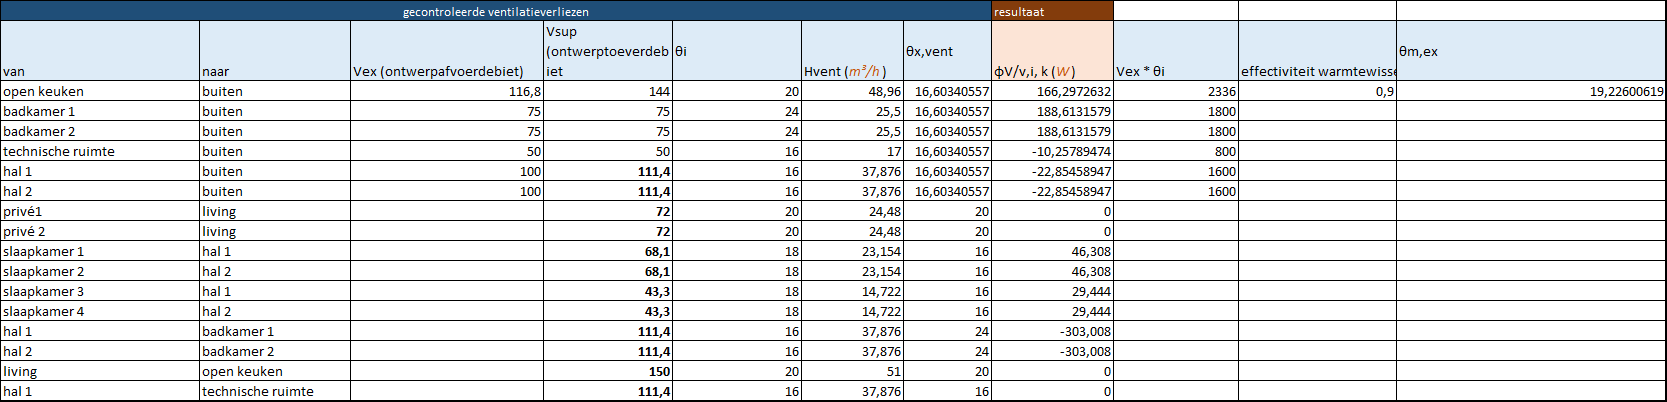
\includegraphics[width=1\linewidth]{gecontroleerdeventilatieverliezen.png}
    \caption{gecontroleerde ventilatieverliezen}
    \label{fig:placeholder}
\end{figure}


\subsubsection{Infiltratie ventilatieverliezen}
De infiltratie verliezen worden berekend per lokaal aan de hand van volgende formule:
\begin{equation}
    \Phi_{inf} = H_{inf} * (\theta_{i} - \theta_{eb})
    \label{eq: infilatratieverliezen}
\end{equation}

met:

\begin{equation}
\begin{aligned}
    &H_{inf} = 0,34 * (0,15*v50*A_t) \\
    &v50 : \text{Het oppervlakte specifiek lekdebiet bij 50} \unit{\pascal} \\
    &A_t = \text{Het warmteverlies oppervlak}
\end{aligned}
\end{equation}
    
De resultaten van deze berekening worden gegeven in figuur \ref{fig:infiltratieverliezen}

\begin{figure}
    \centering
    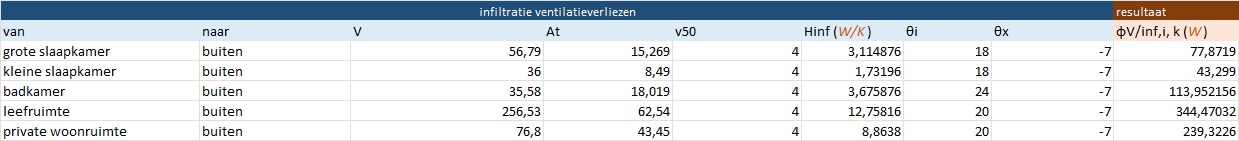
\includegraphics[width=1\linewidth]{infiltratieverliezen.png}
    \caption{infiltratie verliezen}
    \label{fig:infiltratieverliezen}
\end{figure}

\subsection{opwarmingsvermogen}

In dit onderzoek wordt het opwarmvermogen (opwarmtoeslag) buiten beschouwing gelaten bij de berekening van de totale warmteverliezen. Deze keuze is gefundeerd op de huidige technologische ontwikkelingen binnen de klimaatbeheersing. Moderne verwarmingssystemen worden gekenmerkt door een laag dimensioneringsvermogen en het gebruik van geavanceerde regeltechnieken, waardoor piekbelastingen tot een minimum worden beperkt. Het incorporeren van een additioneel opwarmvermogen zou in deze context resulteren in een significante overdimensionering van de warmtepomp, wat de efficiëntie van de installatie nadelig beïnvloedt.

\subsection{Totaal te installeren verwarmingsvermogen}

Het totaal te installeren verwarmingsvermogen ($\Phi_{HL}$) per ruimte vertegenwoordigt de maximale warmtebehoefte waaraan de verwarmingsinstallatie moet voldoen om de gewenste ontwerpbinnentemperatuur te handhaven in ontwerpomstandigheden. Dit nominale vermogen is de som van de berekende transmissieverliezen ($\Phi_T$), de totale ventilatie- en infiltratieverliezen ($\Phi_V$) en een eventueel vereist extra opwarmingsvermogen ($\Phi_{RH}$):

\begin{equation}
    \Phi_{HL} = \Phi_T + \Phi_V + \Phi_{RH}
\end{equation}

Gezien het voorliggende ontwerp gebruikmaakt van een warmtepomp als opwekker, is een continu stookregime op lage temperatuur sterk aangewezen om de efficiëntie (SPF) te maximaliseren en overdimensionering te voorkomen. Nachtverlaging wordt om deze reden vermeden, waardoor het extra opwarmingsvermogen ($\Phi_{RH}$) in deze berekening voor alle lokalen op 0 W is gesteld. De benodigde warmteafgifte per lokaal resulteert zodoende puur uit de compensatie van transmissie- en ventilatieverliezen. Het totale warmteverlies is te zien in Tabel \ref{tab:samenvatting_verliezen}.

\begin{table}[h]
\centering
\begin{tabular}{lr} % l = links uitgelijnd (tekst), r = rechts uitgelijnd (getallen)
\toprule
\rowcolor{gray!20} \textbf{Omschrijving} & \textbf{Waarde [W]} \\ \midrule
Totale transmissieverlies $\phi_{T,i}$ & 4264,06 \\
Totale ventilatieverlies $\phi_{V,i}$  & 442,50 \\ \midrule
\textbf{Totaal warmteverlies $\phi_{HL,i}$} & \textbf{4706,56} \\ \bottomrule
\end{tabular}
\caption{Samenvatting van de totale warmteverliezen.}
\label{tab:samenvatting_verliezen}
\end{table}

\subsection{Evenwichtstemperatuur}


\section{Hydraulisch ontwerp}

\subsection{Leidingstracé}

\subsection{Selectie van radiatoren}
Er wordt gekozen voor een temperatuurregime van 45/35. De meeste technische fiches voor radiatoren worden gegeven aan een regime 75/65/20. Bij het selecteren van de radiatoren wordt hiermee rekening gehouden door correctiefactoren (f1) te gebruiken. In de technische fiche die hier gehanteerd wordt (zie bijlage) staat op p.154 een tabel met correctiefactoren. Naargelang de plaatsing moet ook een correctiefactor gebruikt worden (f2). Aangezien er geen afwijkende opstellingen zijn, is deze factor gelijk aan 1.

Indien het warmteverlies van het lokaal gekend is, weet men ook de benodigde warmteafgifte bij het waterregime dat gehanteerd wordt (45/35). Bijvoorbeeld in de badkamer is een warmteafgifte van 654,1 Watt nodig bij een waterregime van 45/35. De badkamer heeft een binnentemperatuur van 24°C. In de tabel van de correctiefactoren uit de technische fiche vindt men dan een correctiefactor gelijk aan 4,58. Men vermenigvuldigd de benodigde warmteafgifte met de correctiefactor waardoor men dan de genormaliseerde benodigde warmteafgifte vindt (bij een regime 75/65/20). In de badkamer bedraagt de genormaliseerde benodigde warmteafgite 2995.769 Watt. Met deze waarde kan gezocht worden naar een geschikte radiator voor dit lokaal. De radiatoren die hier gekozen worden zijn terug te vinden op p.18-19 in de technische fiche in bijlage. Aangezien de radiatoren onder de ramen geplaatst worden, wordt er telkens rekening gehouden met de hoogte zodat deze niet voor het raam komen te staan. In de badkamer wordt gekozen voor een radiator type 33 met een hoogte van 900 mm een breedte van 1100mm. Eens een radiator gekozen is, kan men dan de werkelijke warmtafgifte gaan berekenen. 
Deze berekeningen worden gedaan voor elke ruimte waar een radiator geplaatst wordt en kan men vinden in volgende tabel: 


\subsection{Waterdebieten}
Het waterdebiet dat door een radiator stroomt kan berekend worden via volgende formule dat te vinden is in het WTCB Rapport 14 (7.3.2.2): 
% Requires: \usepackage{amsmath}
\begin{equation}
    q_{m,\mathrm{rad}} = \frac{\Phi \cdot 3600}{c \cdot \left( \theta_{w,i} - \theta_{w,r} \right)} \quad (\mathrm{kg/h})
    \label{eq:placeholder_label}
\end{equation}
met:
\begin{equation*}
\begin{aligned}
    &\Phi : \text{Het werkelijk afgegeven vermogen van de radiator} \\
    &c : \text{De specifieke warmtecapaciteit van water} \\
    &\theta_{w,i} = \text{Ontwerpvertrektemperatuur} \\
    &\theta_{w,r} = \text{Ontwerpretourtemperatuur} \\
    \\
\end{aligned}
\end{equation*}
Bij een gemiddelde watertemperatuur van 40°C vindt men in tabel A.1 uit het WTCB Rapport 14 dat de waarde van c gelijk is aan 4179 J/kgK \qty{4179}{\joule\per\kilo\gram\per\kelvin} 

De benodigde waterdebieten voor de radiatoren wordt gegeven in volgende tabel:

\subsection{Watersnelheden}

\subsection{Dimensioneren van warmteleidingen}
 Aangezien we voor de radiatoren in de bovenverdieping het waterregime 45/35 gebruiken rekenen we verder met een gemiddelde watertemperatuur van 40°C in de leidingen en een volumemassa van \qty{4179}{\joule\per\kilo\gram\per\kelvin}.
 \begin{figure}
    \centering
    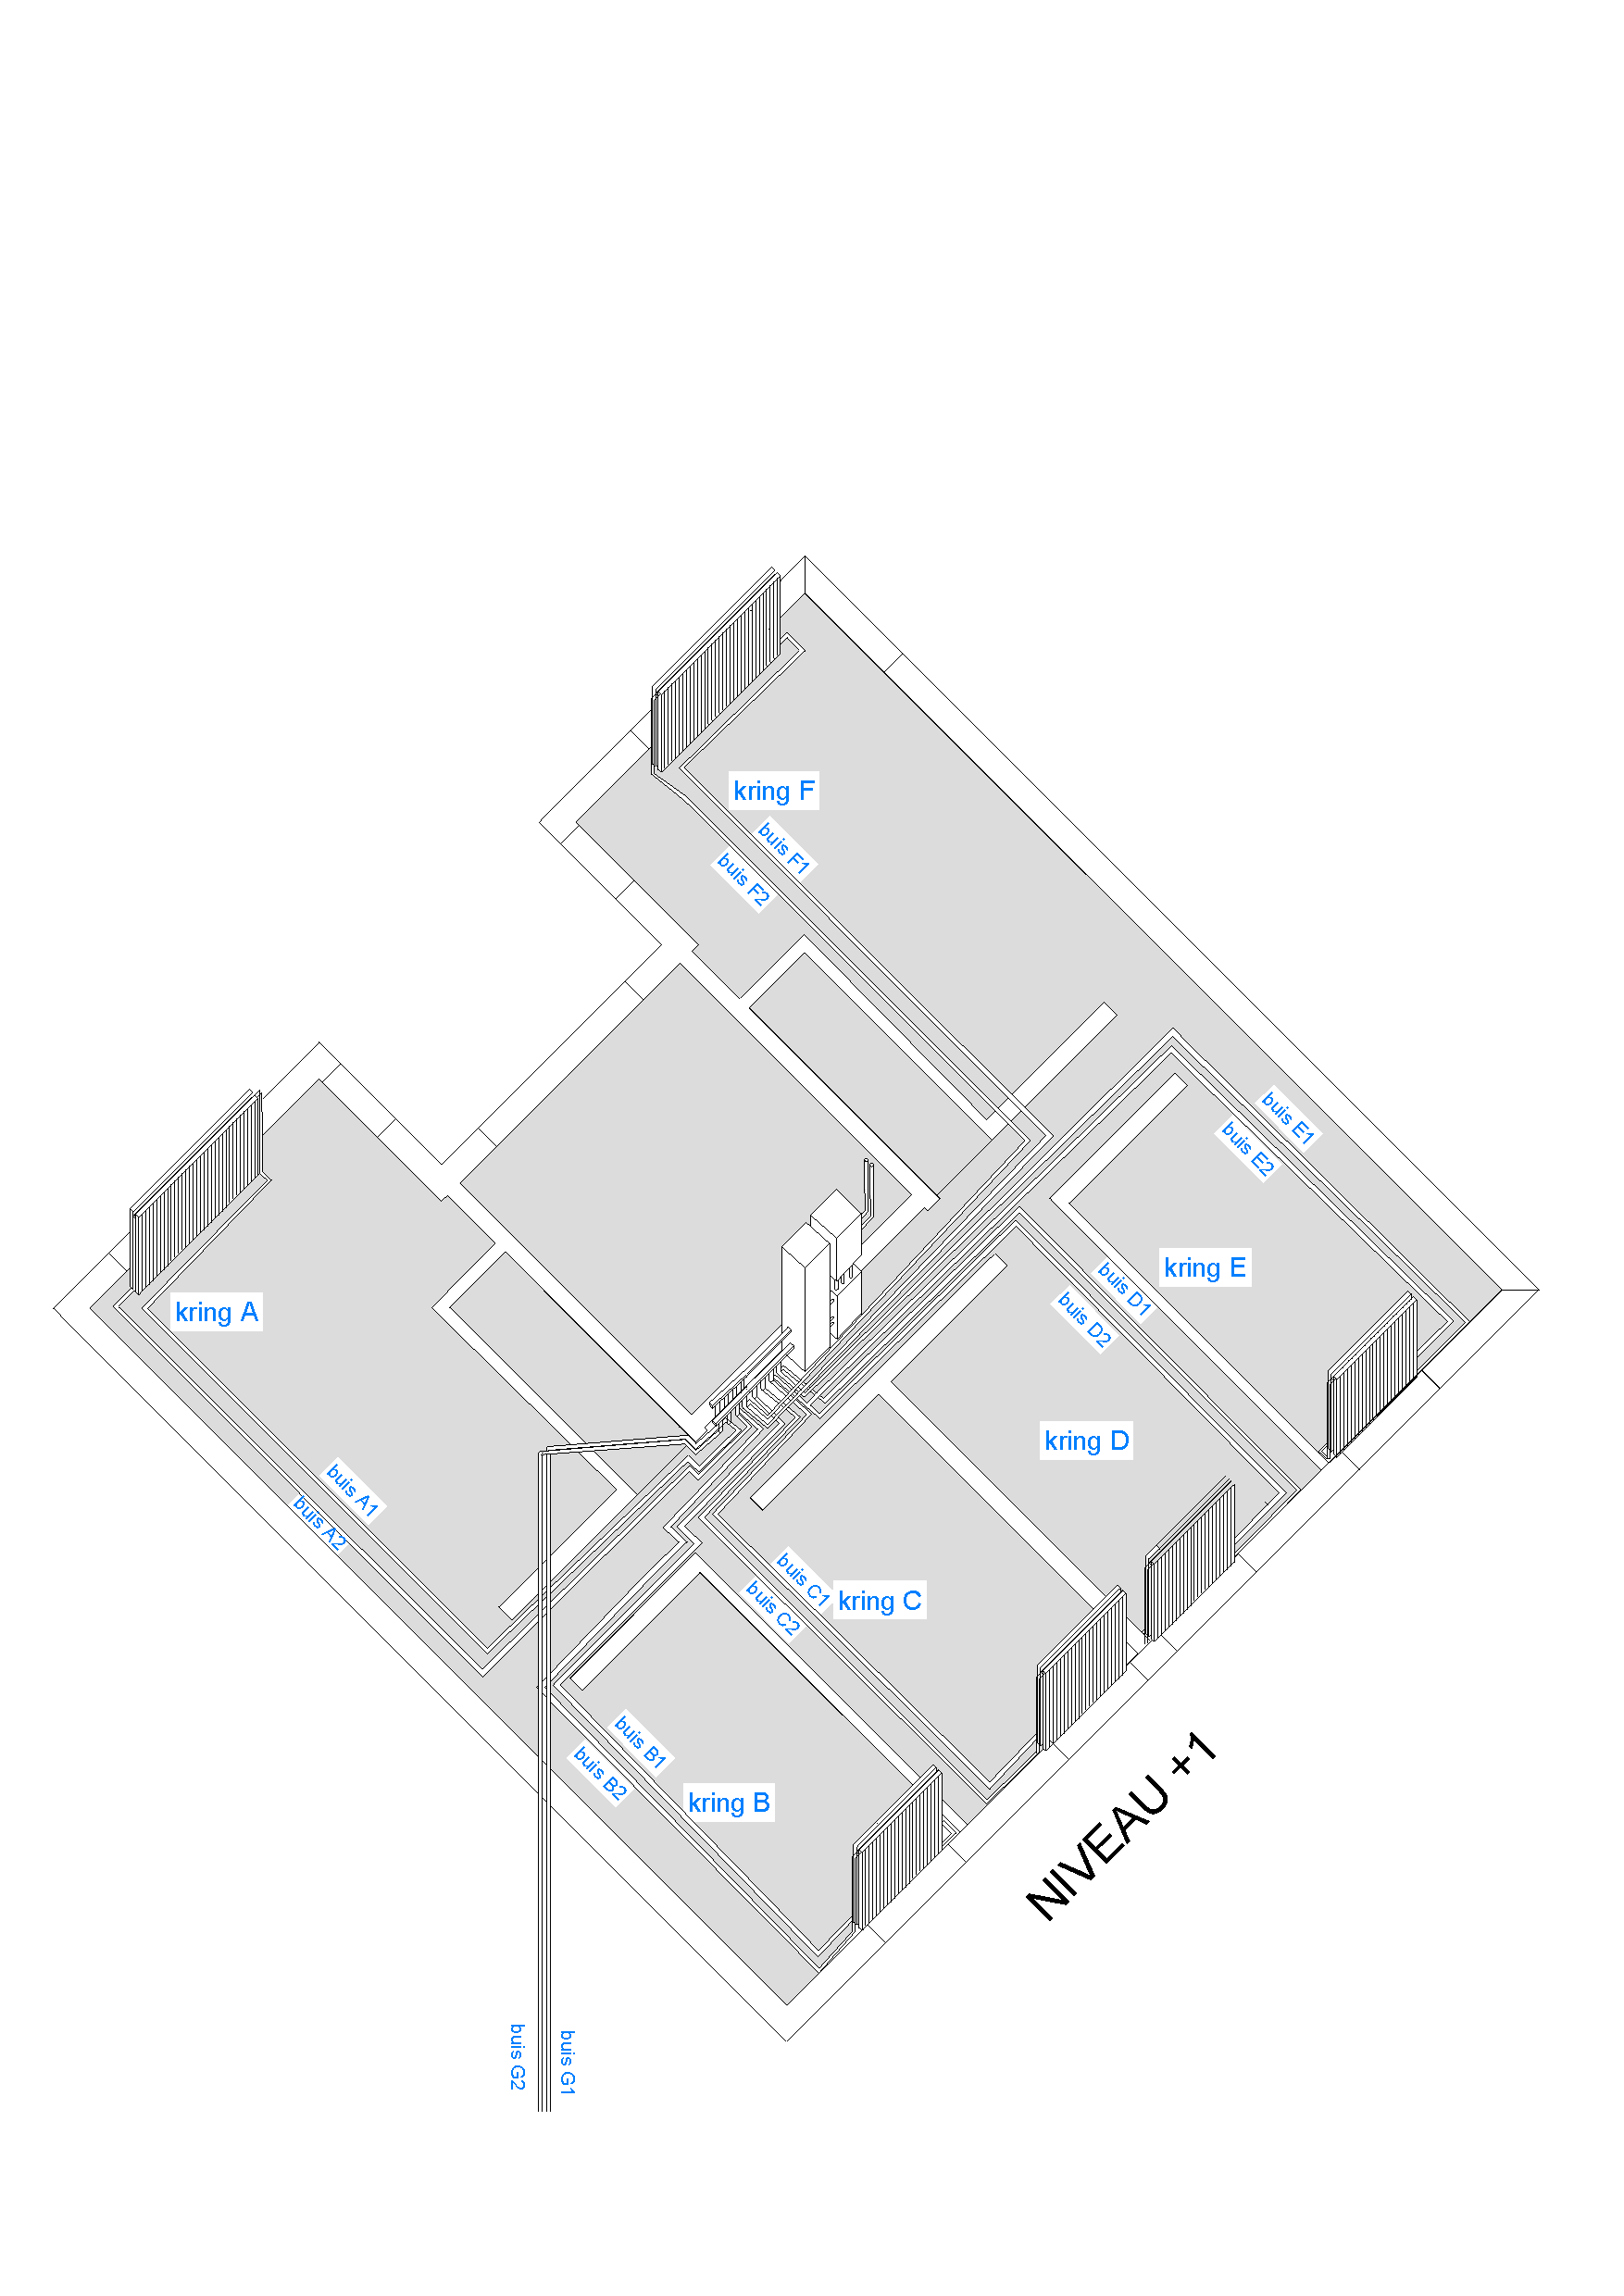
\includegraphics[width=1\linewidth]{figuren/axo TIG leidingen 3.pdf}

    \caption{Axonometrie warmteleidingen}
    \label{fig:axo leidingen}
\end{figure}
Naast de kring naar de vloerverwarming onderscheiden drie verschillende kringen (zie Figuur \ref{fig:axo leidingen}): kring A bedient de radiator in de grote slaapkamer, kring B bedient deze in de kleine slaapkamer en kring C deze in de badkamer. De overige kringen (D, E en F) zijn volledig analoog ten gevolge van de symmetrie van het grondplan.

Bij het bepalen van de binnendiameter van de leidingen rekenen we verder met de bekomen waterdebieten. De formule uit het WTCB Rapport 14 p.94 voor het berekenen van de watersnelheid in een buisstuk hebben we hieronder omgevormd naar de binnendiameter $D_{i}$:
\begin{equation}
    D_i=\sqrt{\frac{q_{m,L}\left(3.54 \cdot 10^{-4}\right)}{v_{max}\rho}}
\end{equation}

\newpage
\appendix
\section{Uitgebreide berekening transmissieverliezen}
\begin{figure}[H]
    \centering
    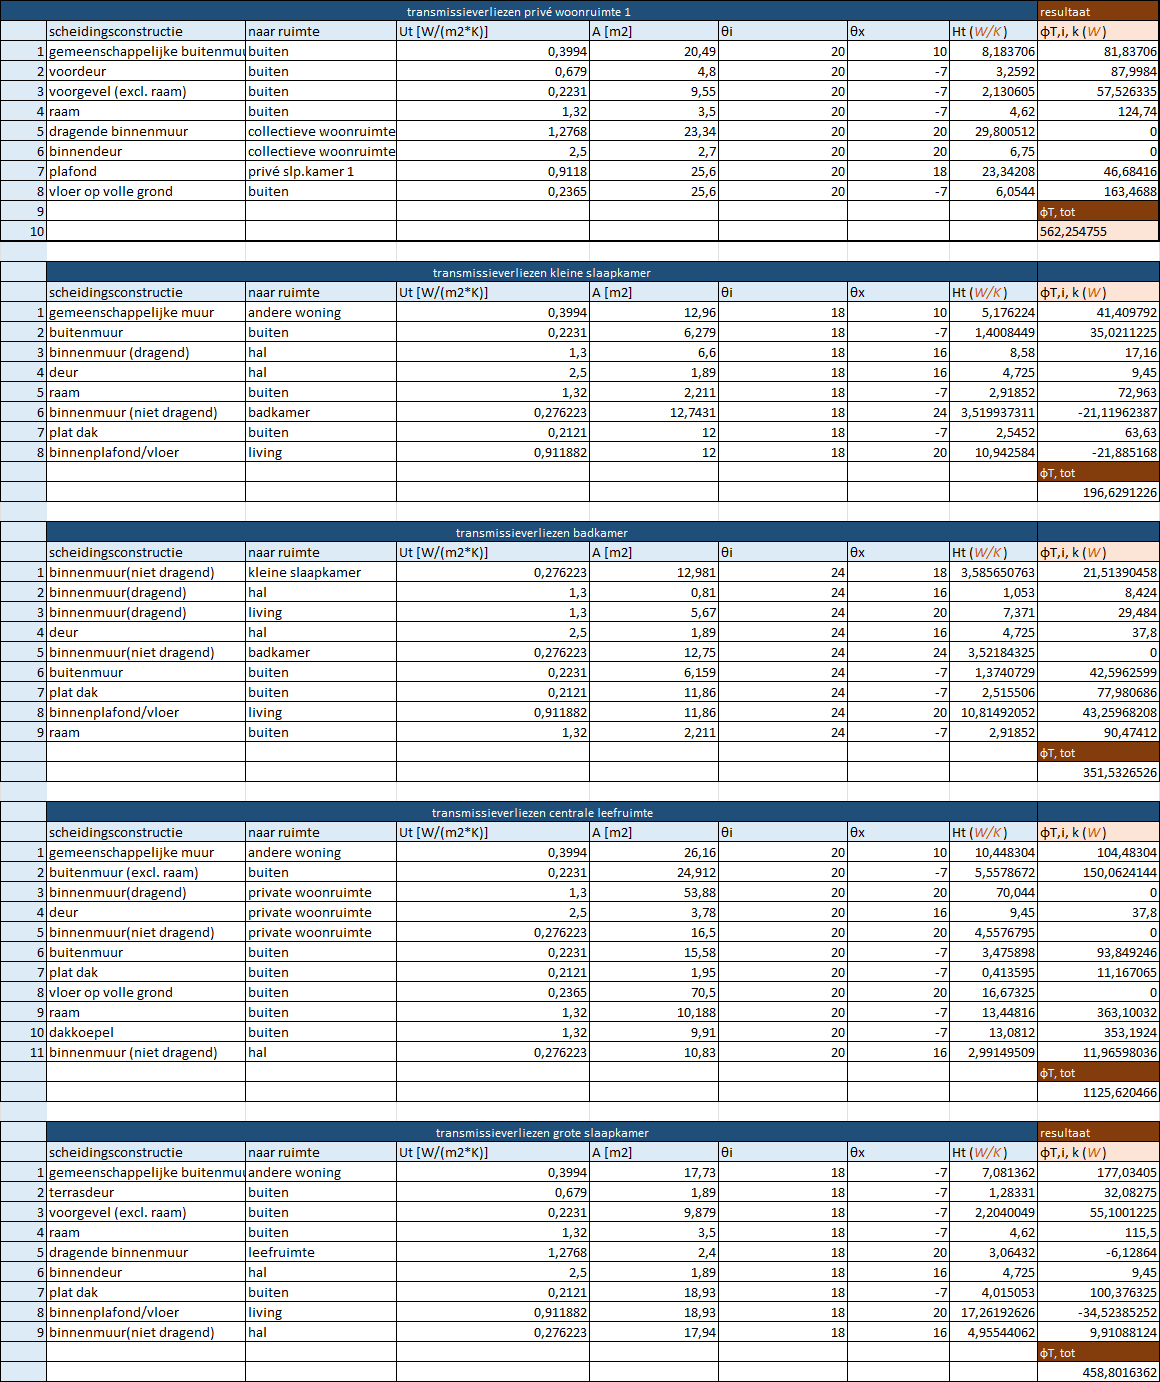
\includegraphics[width=1\linewidth]{alletransmissieverliezen.png}
    \label{fig:placeholder}
\end{figure}

\end{document}
